		\section{Nombre: Lluvia de flechas}\label{obs.lluviaF}
	\subsection{Descripción}
	Lluvia de flechas que se activa cada determinado tiempo y dura un periodo corto de tiempo. No puede atravesar otros obstáculos como plataformas o el suelo. Al hacer contacto con el jugador, reducirá la cantidad de vida del jugador.
	\subsection{Esquema}
Ver figura \ref{fig:lluviaF}.
\begin{figure}
	\centering
	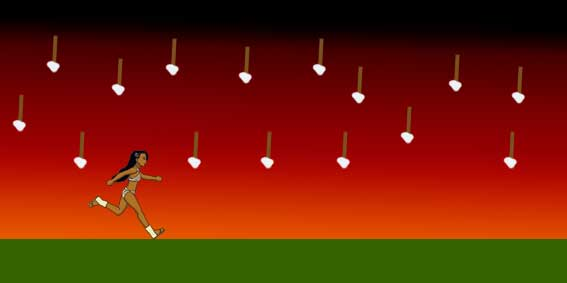
\includegraphics[height=0.3 \textheight]{Imagenes/flechas}
	\caption{Lluvia de flechas.}
	\label{fig:lluviaF}
\end{figure}